\subsection{Round Robin Sorter}

\begin{figure}[h]
    \centering
    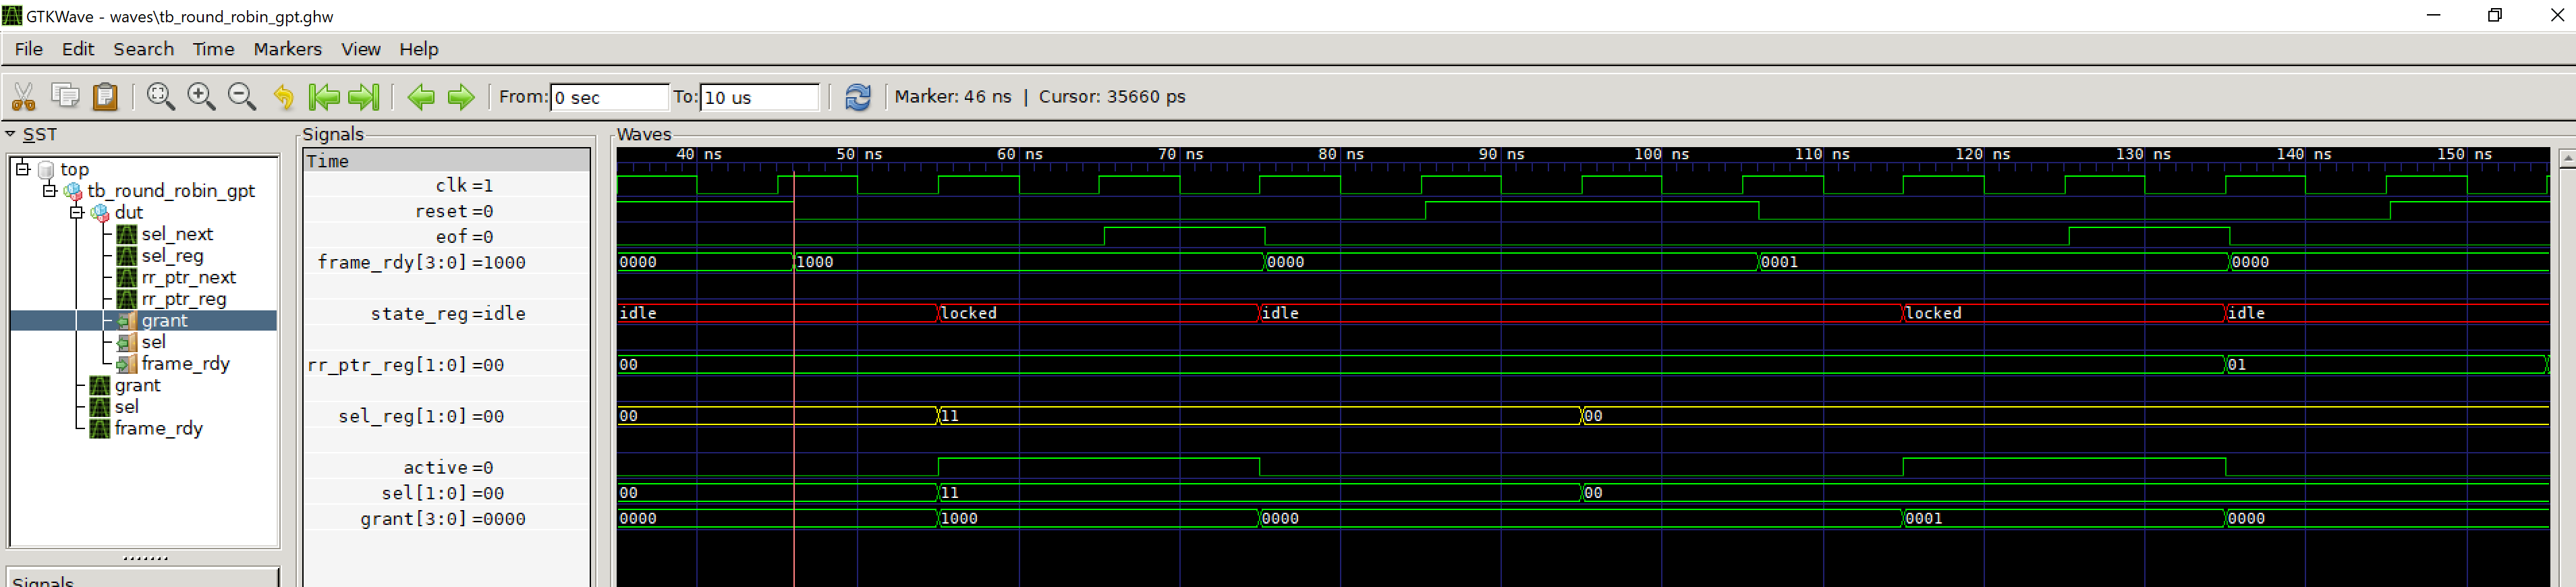
\includegraphics[width=\linewidth]{figures/rr_sorter/RR_wave_test1.PNG}
    \caption{Simulation waveform of the round-robin arbiter showing request detection, lock behaviour, and release on \texttt{eof}.}
    \label{fig:tb_round_robin_wave}
\end{figure}

Figure~\ref{fig:tb_round_robin_wave} shows a section of the simulation of the round-robin arbiter. At the beginning of the shown interval, the arbiter is in the \texttt{IDLE} state, with \texttt{grant = 0000} and \texttt{active = 0}, meaning that no input is currently selected. Around 50\,ns, the request vector changes to \texttt{frame\_rdy = 1000}, so only input port~3 requests service. In the following clock cycle, the arbiter detects this request and changes from \texttt{IDLE} to \texttt{LOCKED}. At the same time, the selected port index becomes \texttt{sel = 11}, which is the binary encoding of input~3, and the one-hot grant output changes to \texttt{grant = 1000}. The signal \texttt{active} also becomes \texttt{1}, indicating that a valid selection is active.

As long as \texttt{eof = 0}, the arbiter remains in the \texttt{LOCKED} state and continues to grant the same port. This can be seen in the waveform between approximately 60\,ns and 75\,ns, where \texttt{sel}, \texttt{grant}, and \texttt{active} remain constant. When \texttt{eof} is asserted, the arbiter releases the current grant. Consequently, the state returns to \texttt{IDLE}, \texttt{grant} returns to \texttt{0000}, and \texttt{active} returns to \texttt{0}. The selected index may still keep its last stored value temporarily, but since \texttt{grant = 0000} and \texttt{active = 0}, no port is considered active anymore.

Later in the waveform, a new request appears with \texttt{frame\_rdy = 0001}, which corresponds to input port~0. Since the arbiter is back in \texttt{IDLE}, it evaluates the new request and again enters the \texttt{LOCKED} state on the next clock edge. The selected index changes to \texttt{sel = 00}, and the grant output becomes \texttt{grant = 0001}. This confirms that the arbiter correctly detects a new request after the previous frame has been completed. Overall, the waveform demonstrates the intended behaviour of the design: the arbiter accepts a request in \texttt{IDLE}, locks to the selected input while the frame is active, and releases the connection when \texttt{eof} is asserted.
\newpage


\begin{figure}[h]
    \centering
    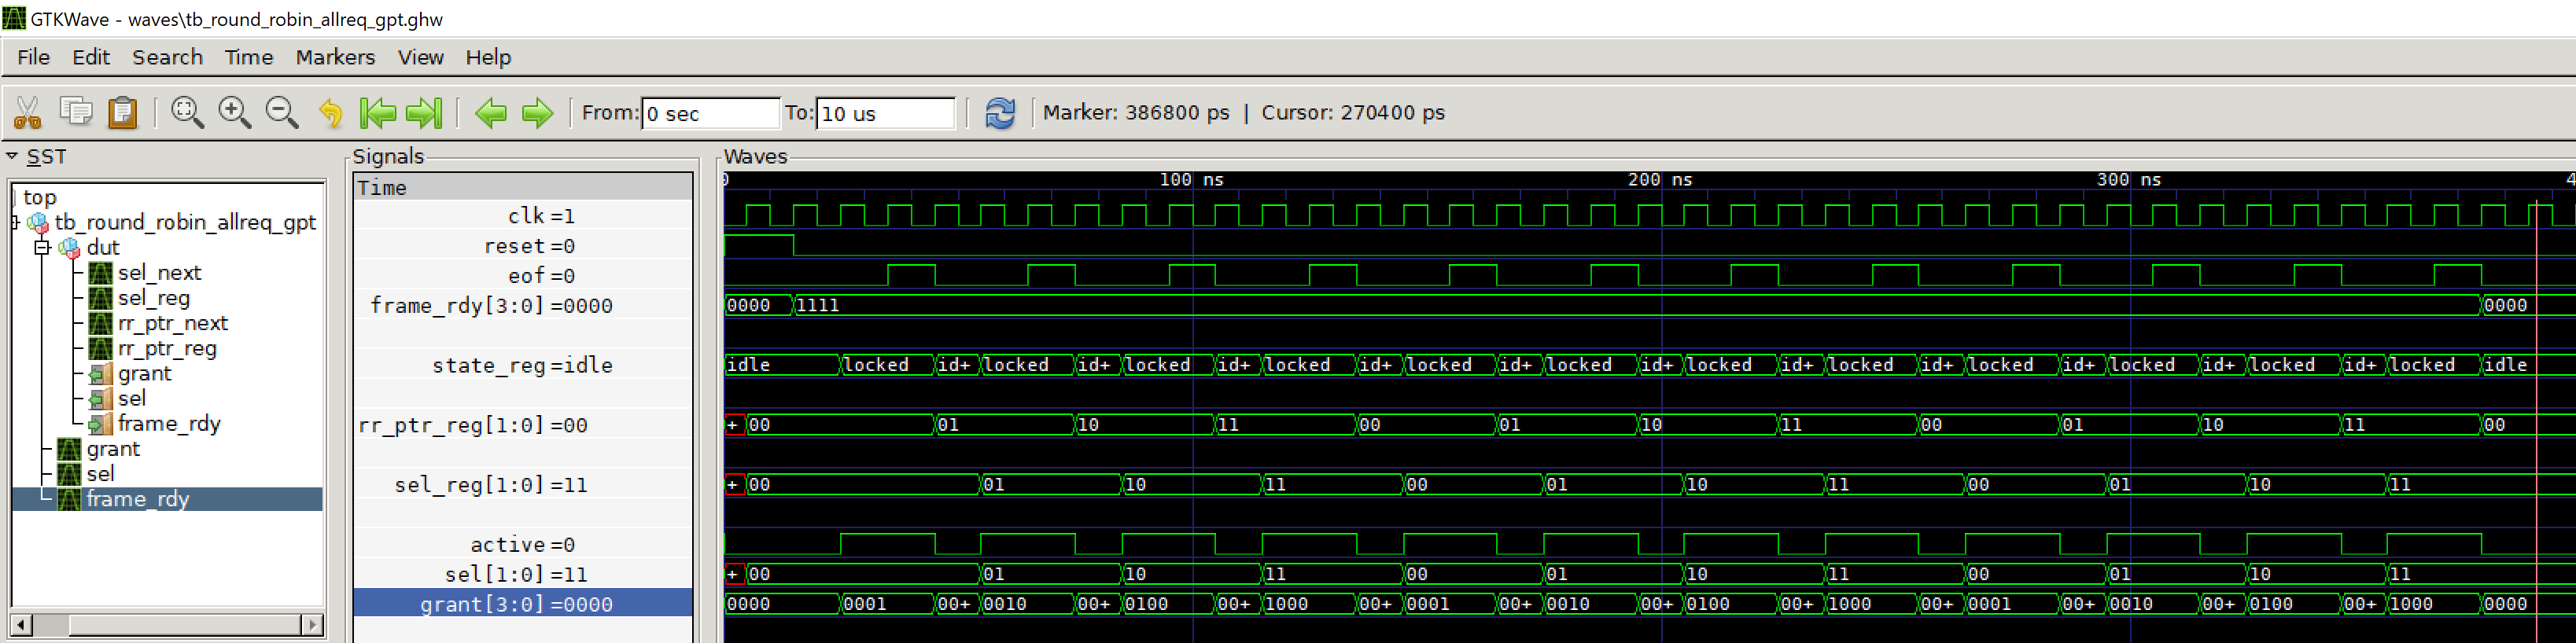
\includegraphics[width=\linewidth]{figures/rr_sorter/RR_wave_test2.PNG}
    \caption{Simulation waveform of the round-robin arbiter showing request detection, lock behaviour, and release on \texttt{eof}.}
    \label{fig:tb_round_robin_wave}
\end{figure}

Figure~\ref{fig:tb_round_robin_wave} shows the simulation of the visualization testbench in which all four request inputs are permanently asserted, i.e.\ \texttt{frame\_rdy = 1111}. The purpose of this test is to clearly demonstrate the cyclic behaviour of the round-robin arbiter. After the reset phase, the arbiter leaves the \texttt{IDLE} state and starts serving one requester at a time. Since all inputs request service continuously, the arbiter always has a valid next candidate available.

Each granted transfer is kept active for two clock cycles while \texttt{eof = 0}. During this time, the state remains \texttt{LOCKED}, the selected binary output \texttt{sel} stays constant, and the one-hot output \texttt{grant} indicates the currently active requester. After these two cycles, \texttt{eof} is asserted for one clock cycle, which causes the arbiter to release the current grant and advance the round-robin pointer to the next requester. As a result, the arbiter repeatedly cycles through all four inputs in the order input~0, input~1, input~2, and input~3.

This behaviour can be seen directly in the waveform. The binary select signal changes in the sequence \texttt{00}, \texttt{01}, \texttt{10}, \texttt{11}, and then repeats. At the same time, the one-hot grant output changes accordingly as \texttt{0001}, \texttt{0010}, \texttt{0100}, and \texttt{1000}. Therefore, the waveform confirms that the arbiter implements the intended round-robin policy correctly and distributes access fairly among all four requesters when they are continuously active. Same applies to \texttt{frame\_rdy = 1011}.

\begin{figure}[h]
    \centering
    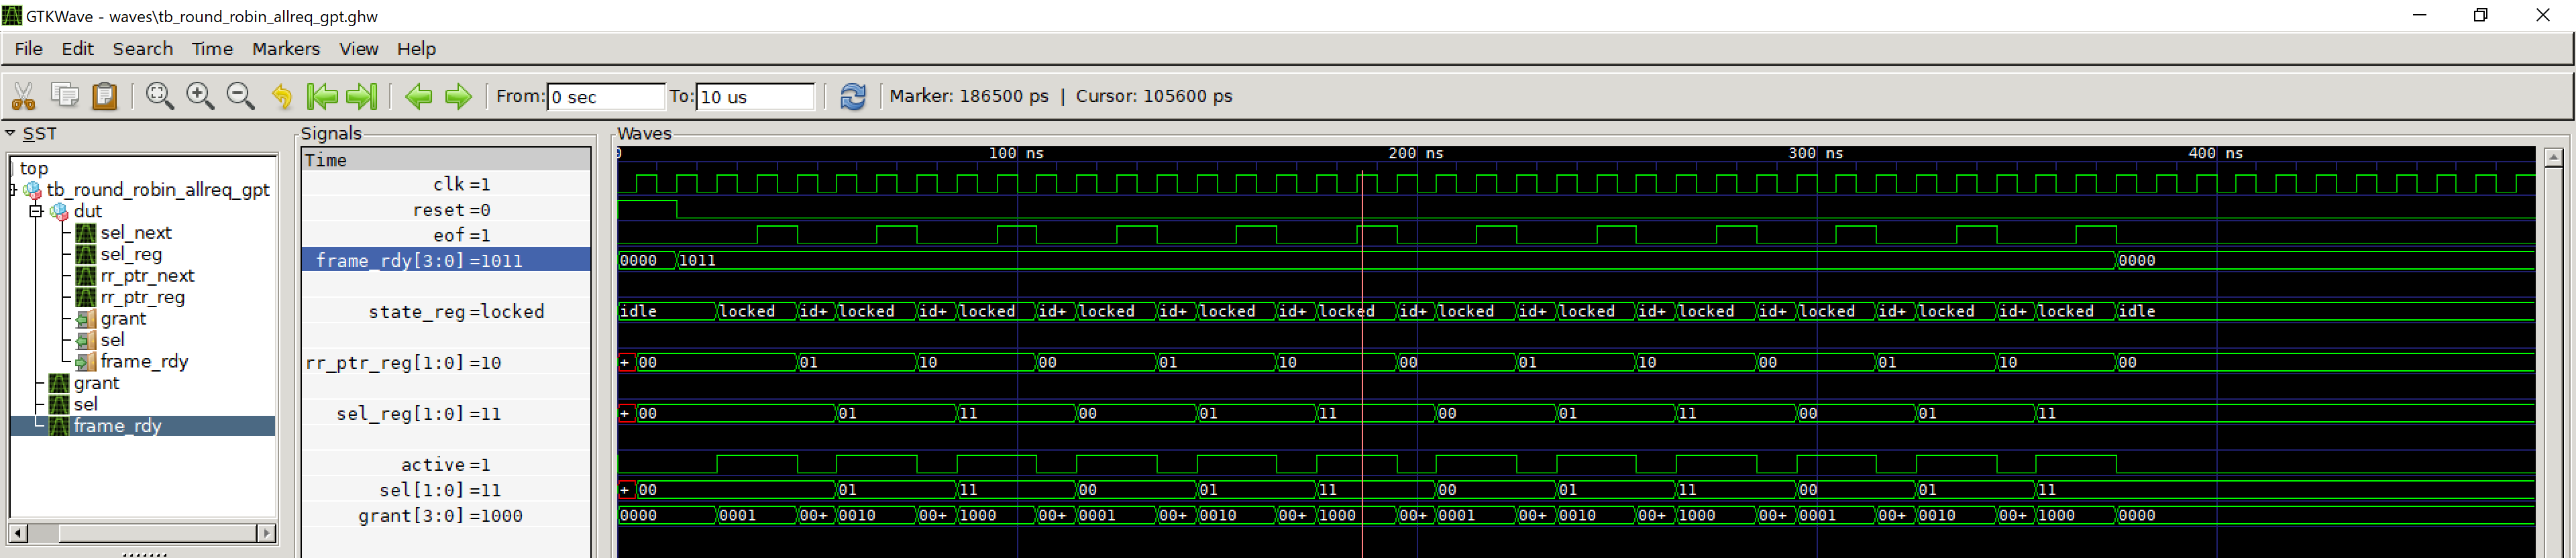
\includegraphics[width=\linewidth]{figures/rr_sorter/RR_wave_test3.PNG}
    \caption{Simulation waveform of the round-robin arbiter showing request detection, lock behaviour, and release on \texttt{eof}.}
    \label{fig:tb_round_robin_wave3}
\end{figure}